\subsection{String resonance angular distributoon}

\begin{figure}[htb]
\begin{center}
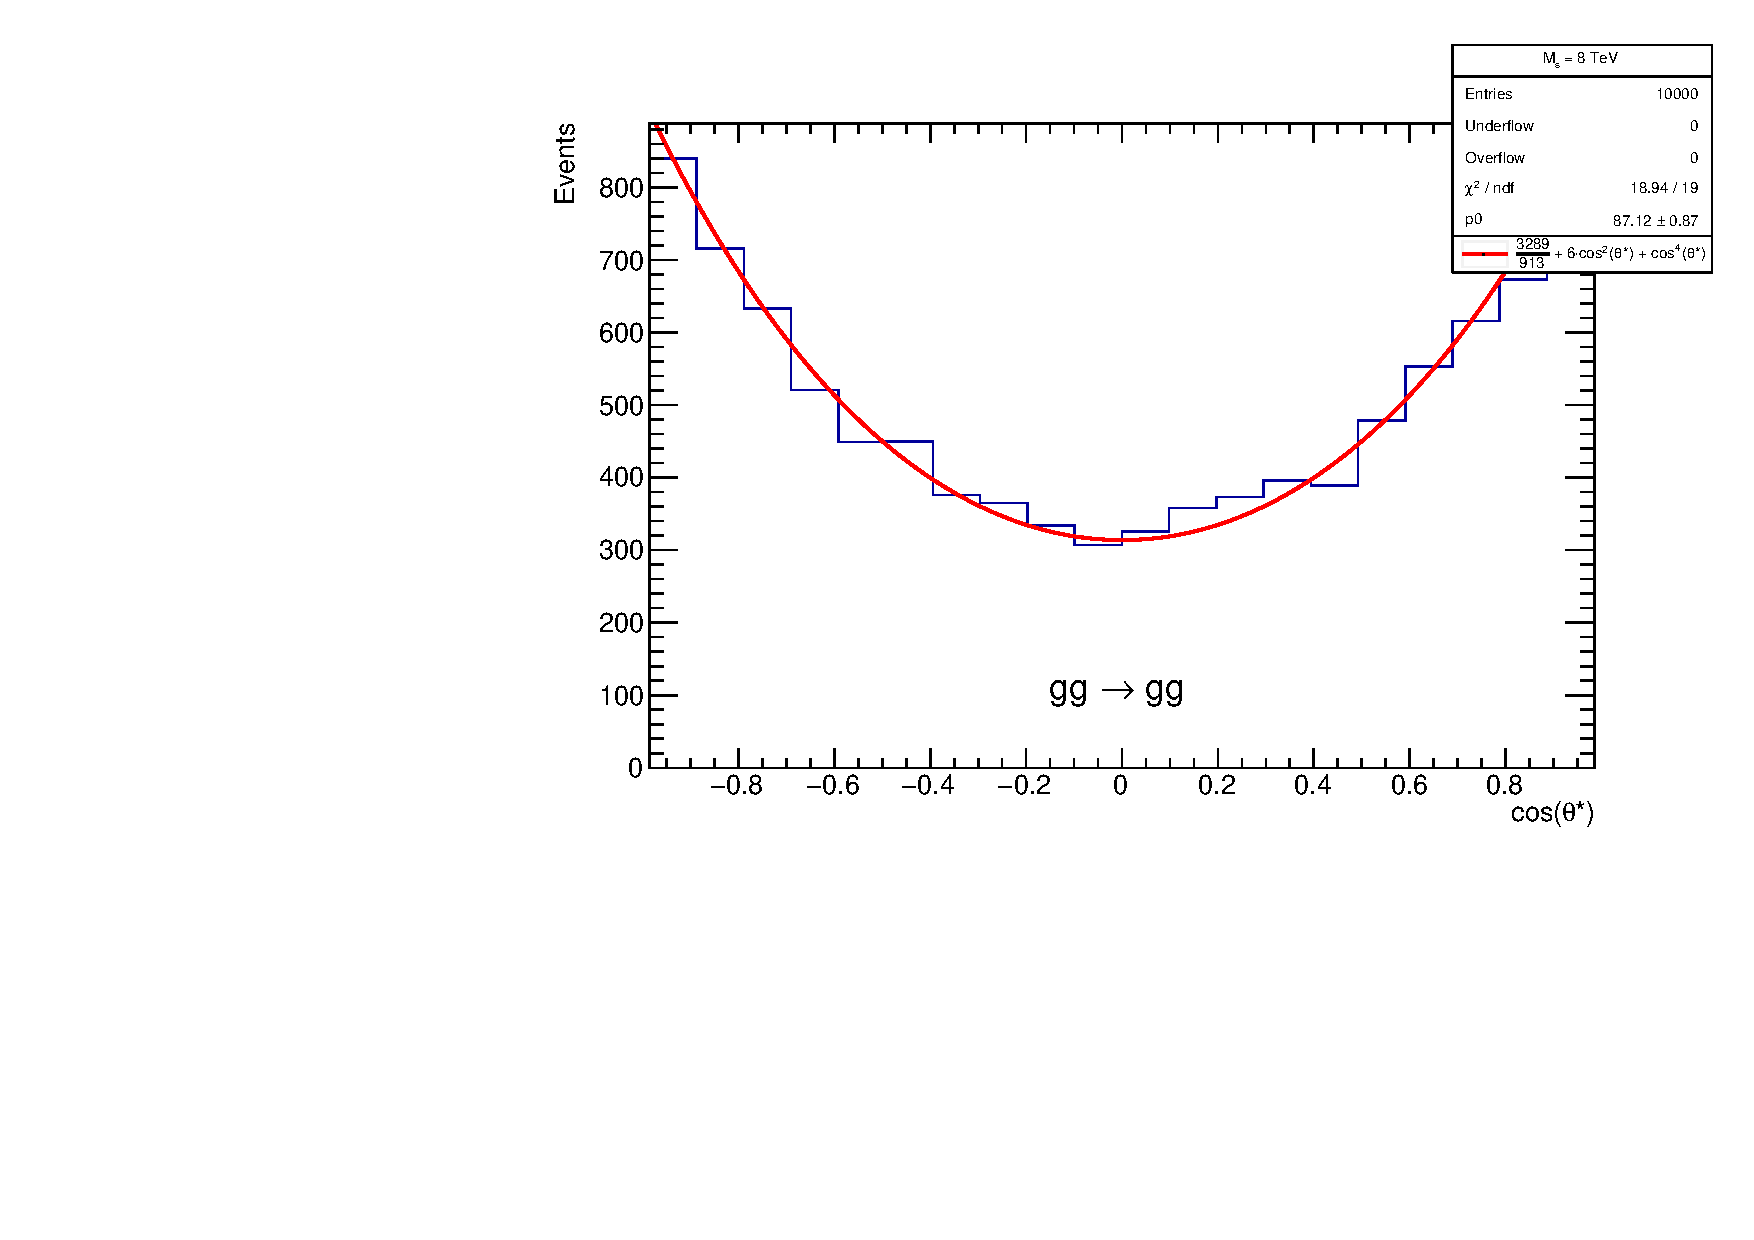
\includegraphics[width=0.45\linewidth]{../figures/strings/angle_gg_gg}
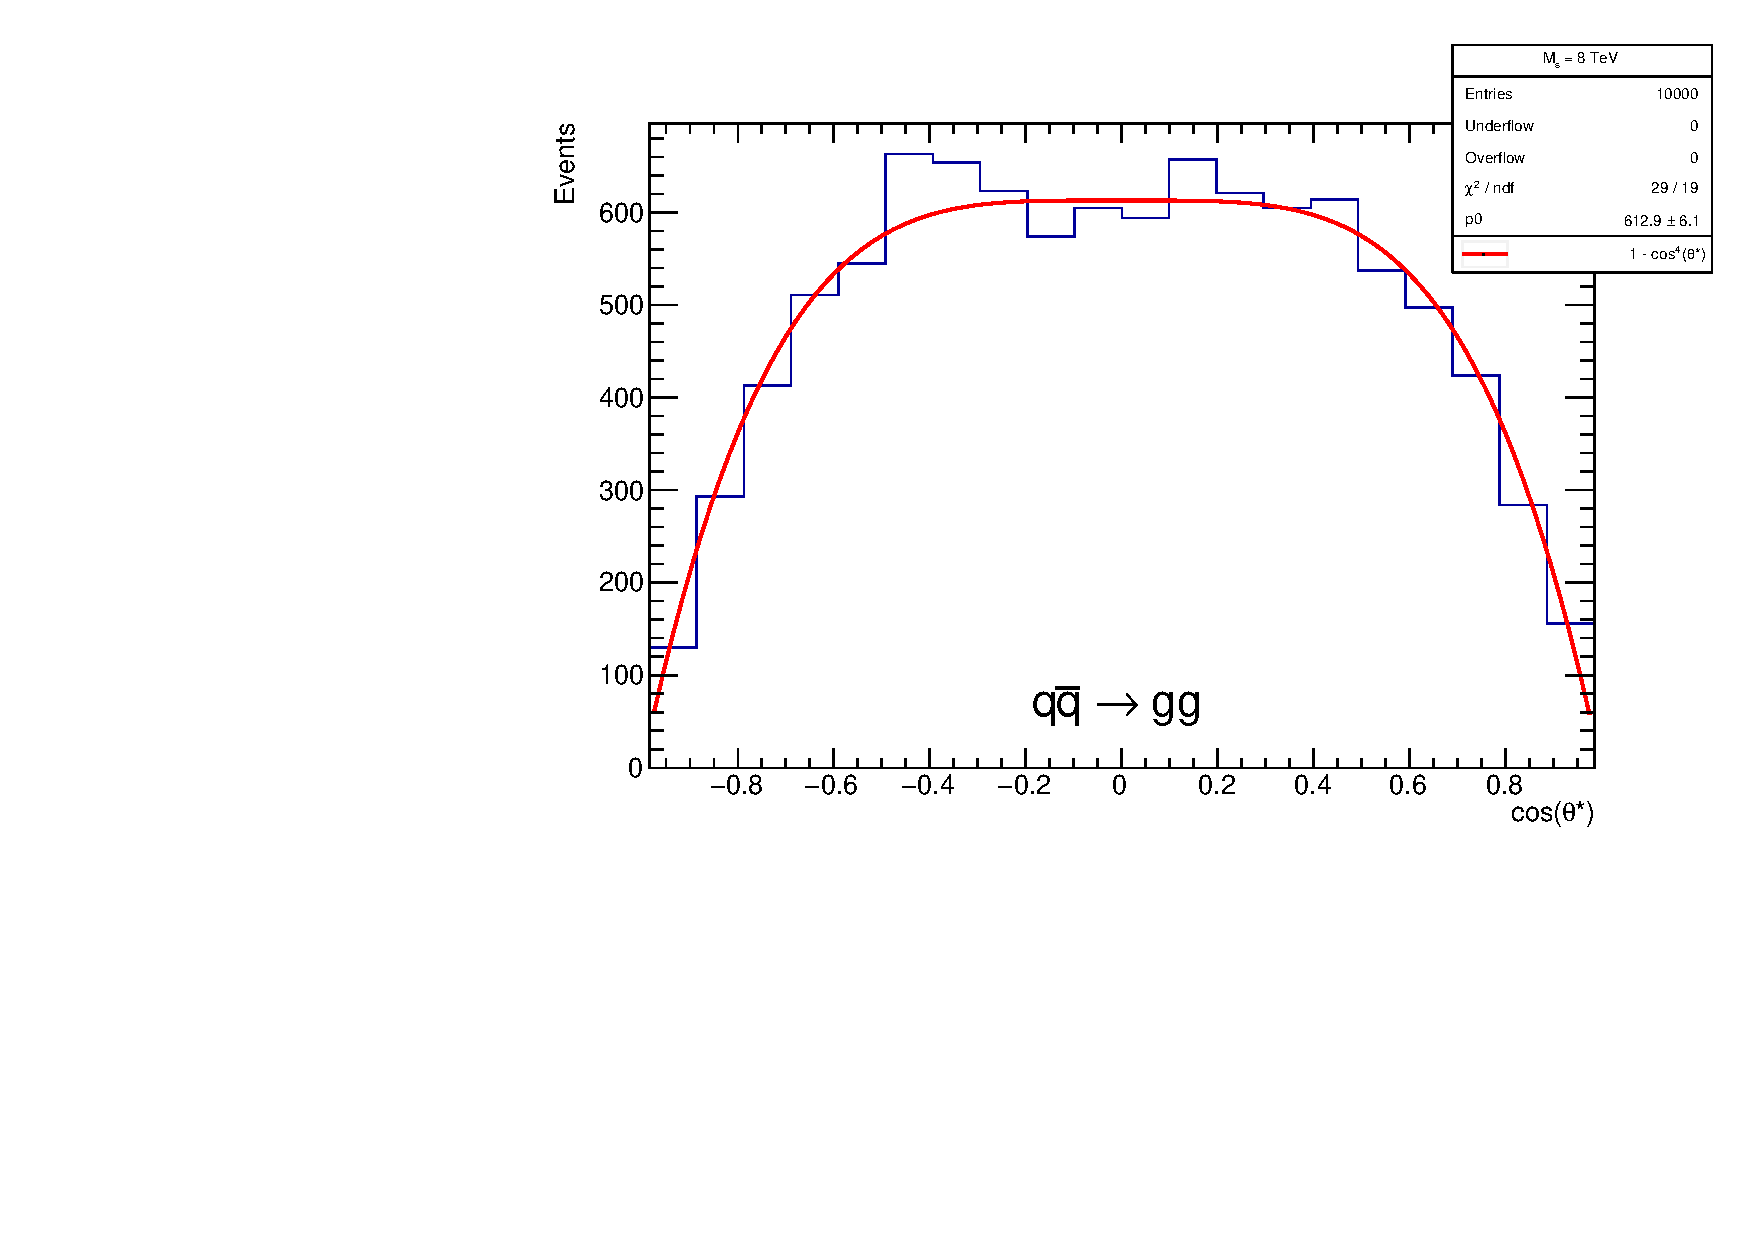
\includegraphics[width=0.45\linewidth]{../figures/strings/angle_qq-bar_gg}
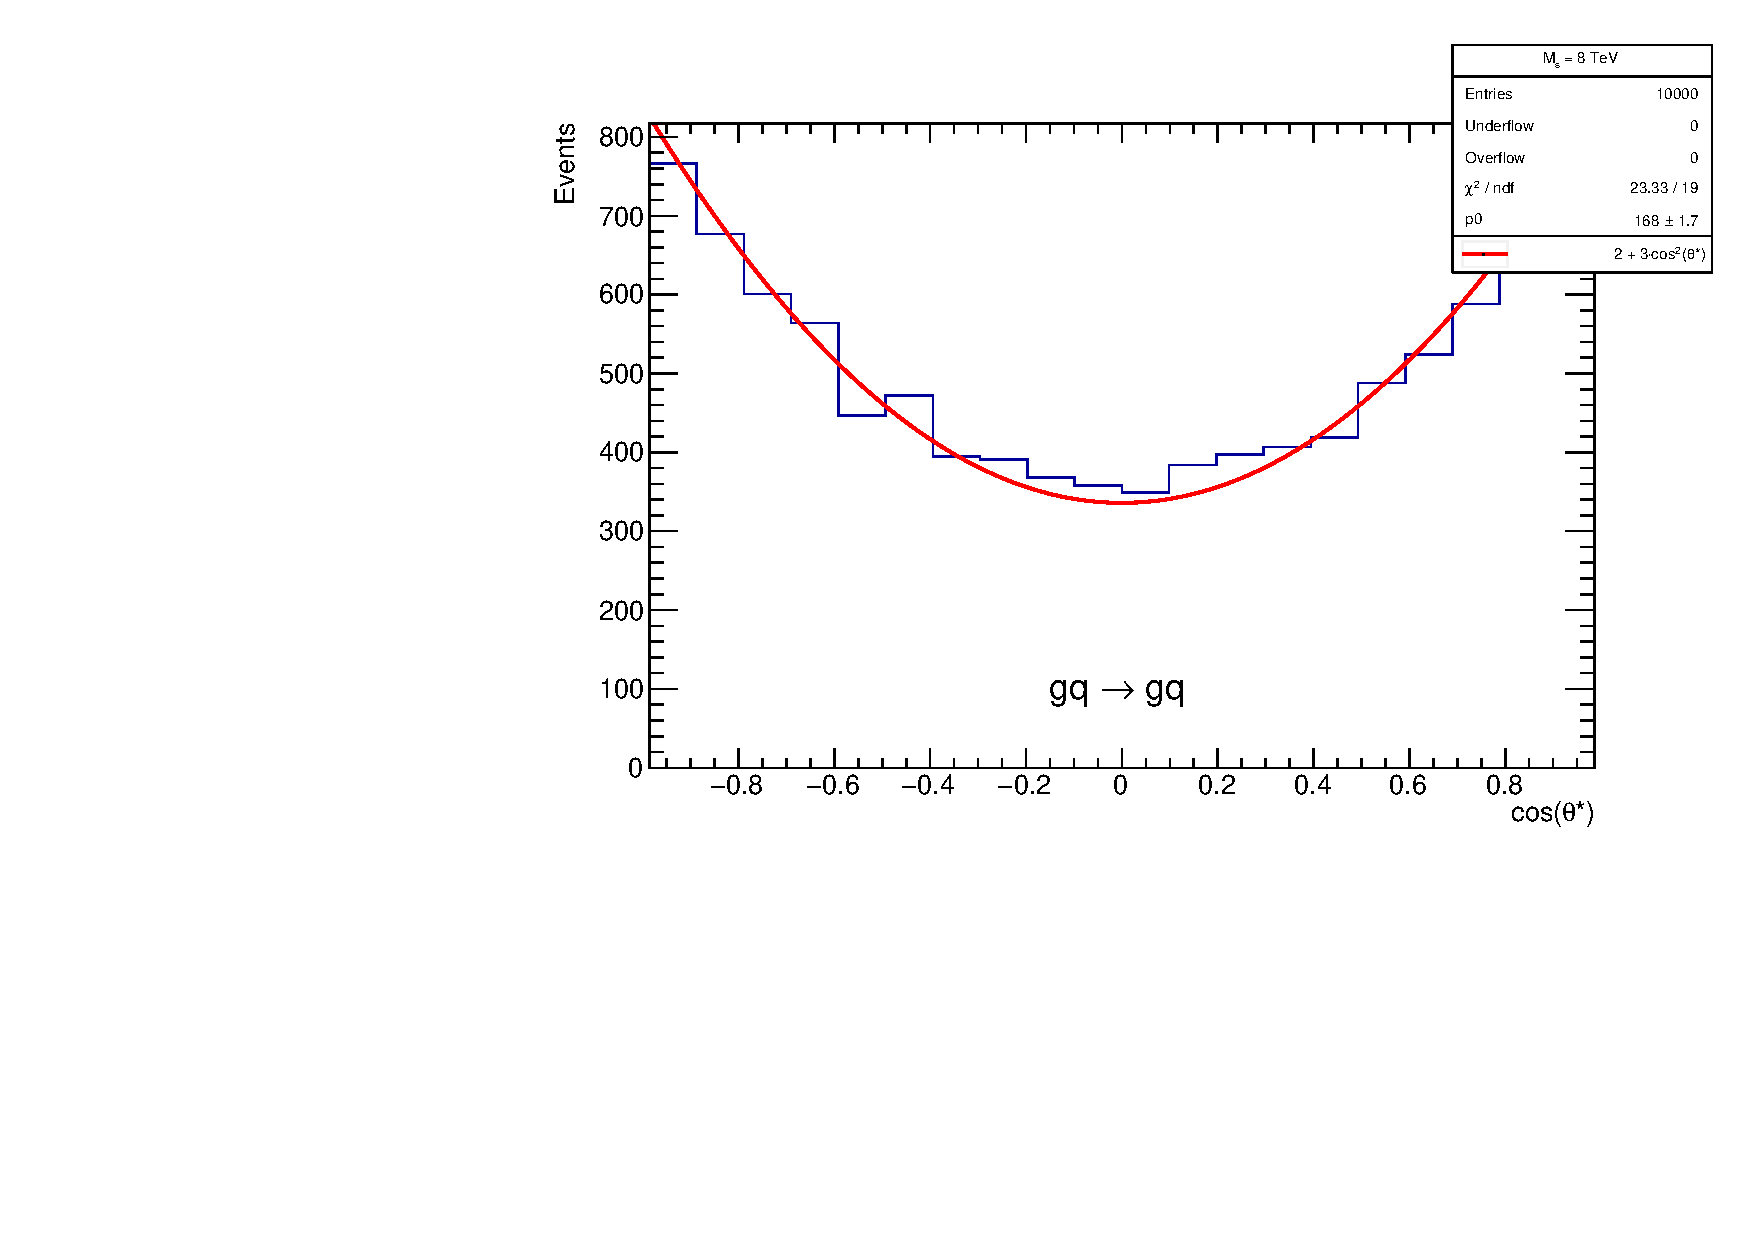
\includegraphics[width=0.45\linewidth]{../figures/strings/angle_gq_gq}
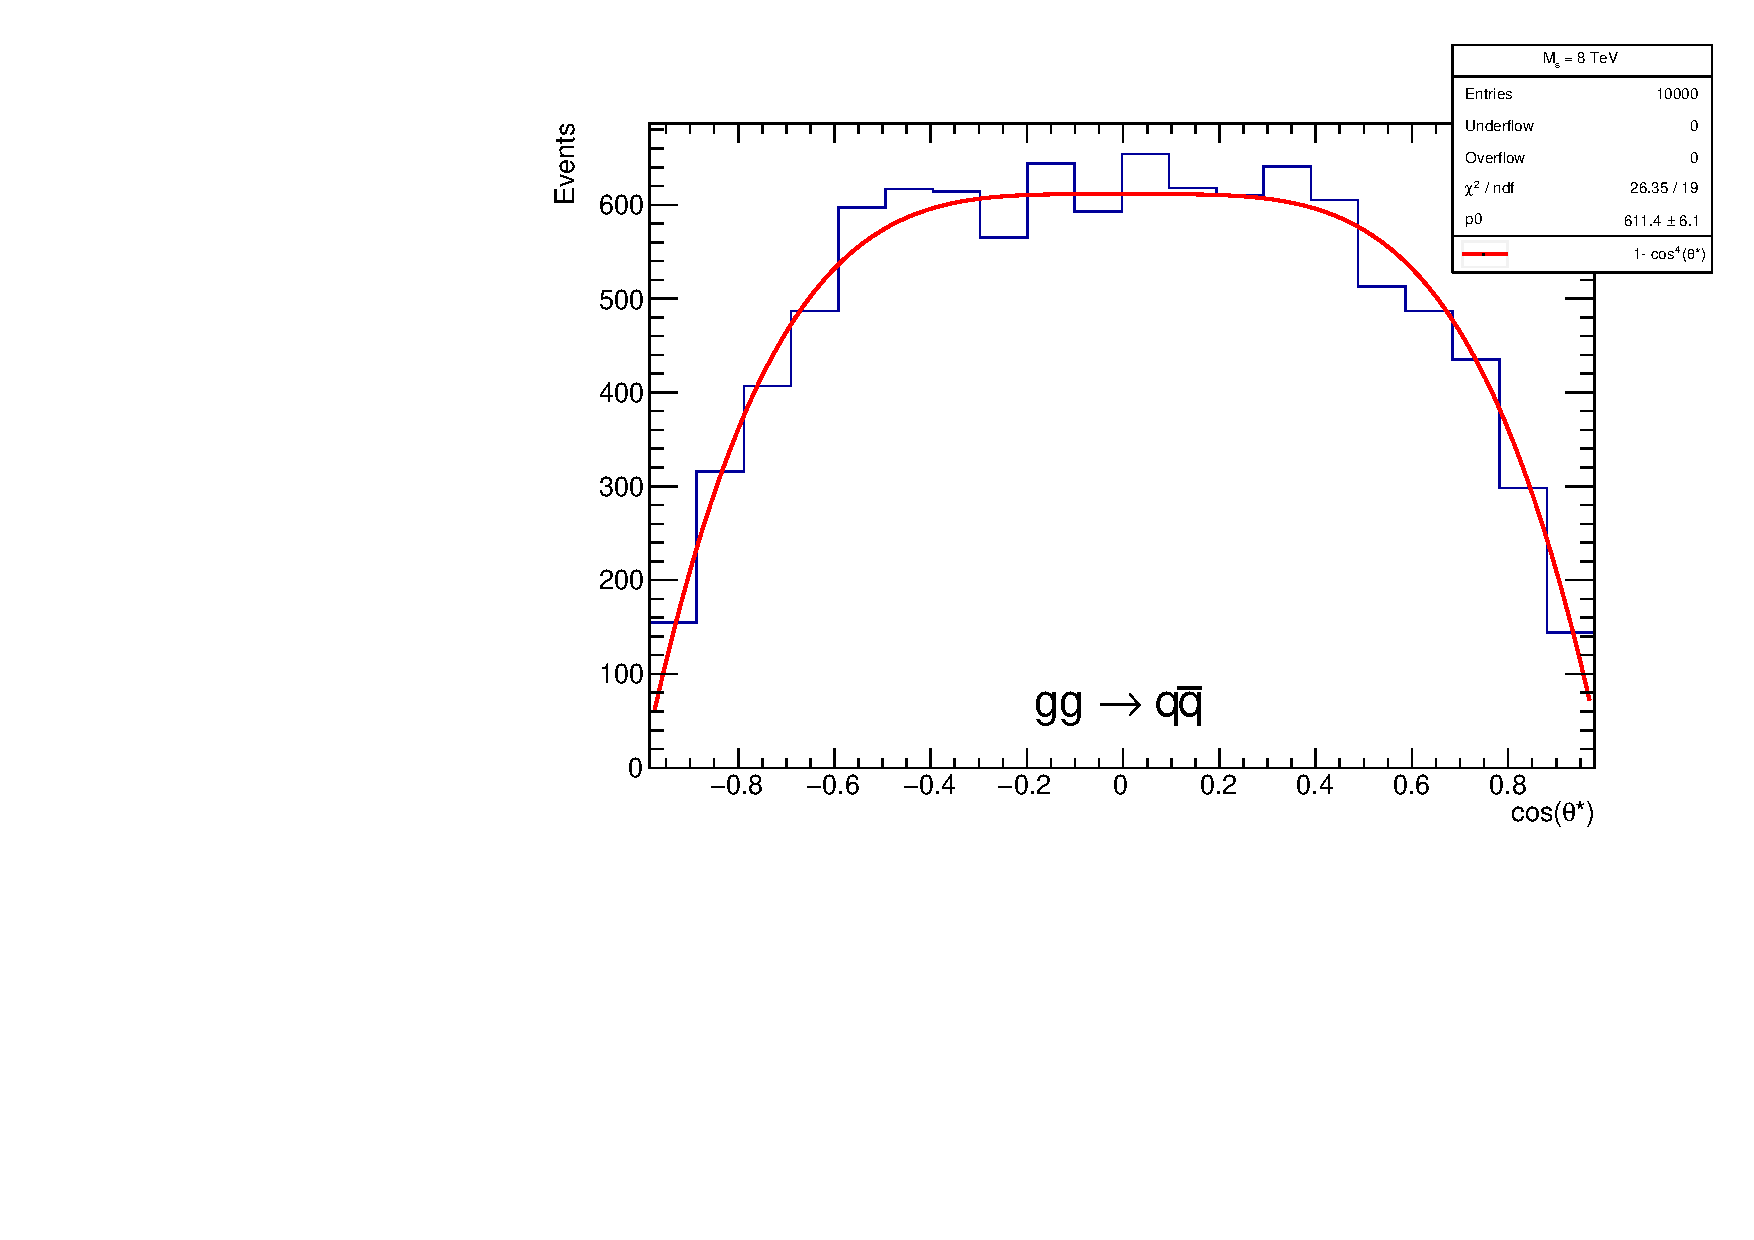
\includegraphics[width=0.45\linewidth]{../figures/strings/angle_gg_qq-bar}
\end{center}
\caption{Angular distribution of the outgoing partons from string
resonances in the centre of mass system: 
(top-left) $gg\to gg$,
(top-right) $q\bar{q}\to gg$,
(bottom-left) $gq\to gq$,
(bottom-right) $gg\to q\bar{q}$.}
\label{fig:stringangle}
\end{figure}

The string resonance consist of a combination excited quark, excited
gluon, and colour singlet states, depending on the subprocess.
In choosing the $y^*$ cut it is useful to examine the decay angular
distributions. 
Figure~\ref{fig:stringangle} shows the angular distribution of the outgoing partons
in the centre of mass system for four different string resonance
subprocesses. 
The case of string scale $\Ms = 8$~TeV is shown but the distributions
are similar for the other generated string scales.
The angular distribution for the process $g\bar{q}\to g\bar{q}$ (not
shown) is similar to $gq\to gq$.
The red curves show the calculated angular distributions for a string
mass equal to \Ms.
